\documentclass{article}
\usepackage{graphicx}
\usepackage[margin = 2cm]{geometry}
\usepackage{caption}
\usepackage{subcaption}

\title{PCO Laboratoire 6 \\
\large Producteur-Consommateur pour calcul différé (Hoare)}
\author{Benoît Delay, Eva Ray}

\setlength{\parskip}{1em}

\begin{document}
\maketitle

\section{Etape 1}
Dans cette étape, nous avons mis en place la distribution des calculs grâce aux méthodes \texttt{requestComputation} et
\texttt{getWork}.

\subsection{Choix d'implémentation}
Pour représenter le buffer contenant les calculs à réaliser, nous avons choisi d'utiliser une map ayant comme clé le
type du calcul et comme valeur une \texttt{std::list} contenant les calculs sous forme de \texttt{Request} à réaliser de
ce type.
Notre
technique consiste simplement à ajouter les calculs au début de la liste correspondante dans la map dès que
\texttt{requestComputation} est appelée.
Cependant, chaque liste a une taille maximale définie par la constante \texttt{MAX\_TOLERATED\_QUEUE\_SIZE}. Pour
modéliser cette contrainte, nous avons créé un tableau nommé \texttt{fullQueuePerType} contenant une \texttt{Condition}
pour chaque type de calcul.
Avant d'ajouter le calcul à la liste, on vérifie donc que la taille de la liste est inférieure à \texttt{MAX\_TOLERATED\_QUEUE\_SIZE}.
Si ce n'est pas les cas, on appelle la fonction \texttt{wait} sur la condition correspondante dans \texttt{fullQueuePerType
} et on attend qu'un calcul du bon type arrive dans le buffer.
La méthode \texttt{requestComputation} est aussi en charge de donner un indice unique à chaque calcul. Pour cela,
nous avons utilisé un attribut statique \texttt{nextId} qui est incrémenté à chaque fois qu'un calcul est ajouté au
buffer.

La méthode \texttt{getWork}, quant à elle, demande du travail d'un certain type. Pour cela, elle vérifie que la liste
correspondante dans la map n'est pas vide. Si c'est le cas, elle appelle la méthode \texttt{pop\_back} sur la liste
afin de récupérer le dernier élément de la liste, qui sera donc le plus ancien. Si la liste est vide, elle appelle la
méthode \texttt{wait} sur la condition correspondante dans \texttt{emptyQueuePerType} qui est un autre tableau
contenant une \texttt{Condition} pour chaque type de calcul qui représente le fait qu'il n'y a pas de calcul de ce
type dans le buffer. Dans ce cas, on attented donc qu'un calcul de ce type soit ajouté au buffer avant de pouvoir
continuer.

Lorsqu'un calcul est ajouté au buffer dans la méthode \texttt{requestComputation}, on signale sur la condition correspondante
dans \texttt{emptyQueuePerType} que le buffer contient maintenant un calcul de ce type. De même, lorsqu'un calcul est
retiré du buffer dans la méthode \texttt{getWork}, on signale sur la condition correspondante dans \texttt{fullQueuePerType}
que le buffer contient maintenant un calcul de ce type en moins.

\subsection{Tests}
L'environnement de test comporte 3 types de calculs différents, 2 calculateurs de type \texttt{A}, un
calculateur de type \texttt{B} et un calculateur de type \texttt{C}. Les calculs de type \texttt{A} sont plus longs
que les calculs de type \texttt{B} qui sont eux même plus longs que les calculs de type \texttt{C}.

\pagebreak

\begin{itemize}
    \item Les Google tests globaux et ceux concernant l'étape 1 passent tous.
    \item Si on envoie une demande de calcul de type \texttt{A}, une calculateur de type \texttt{A} prend le calcul.
    C'est le comportement attendu.
    \item Si on envoie 3 demandes de calcul de type \texttt{A}, les 2 calculateurs de type \texttt{A} prennent 2
    calculs, le troisième est en attente jusqu'à ce qu'un calculateur de type \texttt{A} ait fini son calcul, celui
    -ci s'occupe alors du troisième calcul. C'est le comportement attendu.
    \item Si on envoie une demande de calcul de type \texttt{A}, une demande de calcul de type \texttt{B} et une
    demande de calcul de type \texttt{C}, 3 calculateurs du bon type prennent chacun un calcul. C'est le comportement attendu.
    \item Si on envoie une demande de calcul de type \texttt{A} alors que la queue du type \texttt{A} est pleine, il
    faut attendre qu'une place se libère dans la queue pour pouvoir ajouter le calcul et que celui-ci ait un
    identifiant. C'est le comportement attendu.
    \item Lorsqu'on envoie des demandes de calculs, un id leur est attribué dans leur ordre d'arrivée en partant de
    0. Ceci peut être vérifié en regardant les logs. C'est le comportement attendu.
\end{itemize}

\section{Etape 2}
Dans cette étape nous avons mis en place la gestion des résultats grâce aux méthodes \texttt{getNextResult} et
\texttt{provideResult}.

\subsection{Choix d'implémentation}
Pour représenter la structure contenant les résultats, nous avons choisi d'utiliser une \texttt{std::list} contenant les
résultats sous forme de \texttt{ResultWithId}. \texttt{ResultWithId} est une structure que nous avons rajoutée
contenant un id et un résultat qui est optionel (grâce à \texttt{std::optional}). Ainis, nous pouvons ajouter le
résultat dans la liste directement après avoir envoyé la requête au calculateur, même lorsque le résultat est encore
en cours de calcul, ce qui nous permet de connaître l'ordre des calculs en cours ou terminé à tout moment. Dans les
faits, un résultat est ajouté à la liste dès que \texttt{requestComputation} est appelée.

La méthode \texttt{getNextResult} est en charge de récupérer le résultat le plus ancien dans la liste. Pour cela, elle
n'as donc qu'à accéder au dernier élément contenu dans la liste. Si la partie optionelle du résultat est vide, cela
signifie que le résultat n'est pas encore disponible et donc que le calcul est toujours en cours. Dans ce cas, on
appelle la méthode \texttt{wait} sur la condition \texttt{notExpectedResult}. Cette dernière est une condition qui
représente le fait que le prochain résultat n'est pas encore disponible. On attend donc que le résultats attendu
soit disponible dans la liste avant de pouvoir continuer. Lorsque c'est le cas, on retire le résultat de la liste et
on le retourne.

La méthode \texttt{provideResult} permet au calculateur de retourner le résultat du calcul. Pour cela, elle cherche
l'id du résultat donné dans la liste \texttt{results} et met à jour la partie optionelle du résultat avec le résultat
donné. Ensuite, elle signale sur la condition \texttt{notExpectedResult} que le prochain résultat est disponible.


\subsection{Tests}
L'environnement de test comporte 3 types de calculs différents, 2 calculateurs de type \texttt{A}, un
calculateur de type \texttt{B} et un calculateur de type \texttt{C}. Les calculs de type \texttt{A} sont plus longs
que les calculs de type \texttt{B} qui sont eux même plus longs que les calculs de type \texttt{C}.

\begin{itemize}
    \item Les Google tests concernant l'étape 2 passent tous.
    \item Si on envoie une demande de calcul de type \texttt{A}, une calculateur de type \texttt{A} prend le calcul
    puis renvoie le résultat lorsqu'il est calculé. C'est le comportement attendu.
    \item Si on envoie 3 demandes de calcul de type \texttt{B}, le calculateur de type \texttt{B} s'occupe des calculs
    dans l'ordre d'arrivée puis renvoie le résultat à chaque fois qu'il est calculé. C'est le comportement attendu. (
    Voir figure 1.a.)
    \item Si on envoie à la suite un calcul de type \texttt{A}, un calcul de type \texttt{B} et un calcul de type
    \texttt{C}, les résultats sont renvoyés dans l'ordre A, B, C, bien que le calcul de type \texttt{C} se soit terminé
    avant le calcul de type \texttt{B}, qui s'est terminé avant le calcul de type \texttt{A}. C'est le comportement
    attendu. (Voir figure 1.b.)
    \item Si on envoie à la suite un calcul de type \texttt{A} et 4 calculs de type \texttt{C}, les calculs de type \texttt{C}
    se terminent avant le calcul de type \texttt{A} mais le résultat du calcul de type \texttt{A} est renvoyé avant.
    C'est le comportement attendu. (Voir figure 1.c.)
\end{itemize}

\begin{figure}[h]
    \begin{subfigure}{0.45\textwidth}
        \centering
        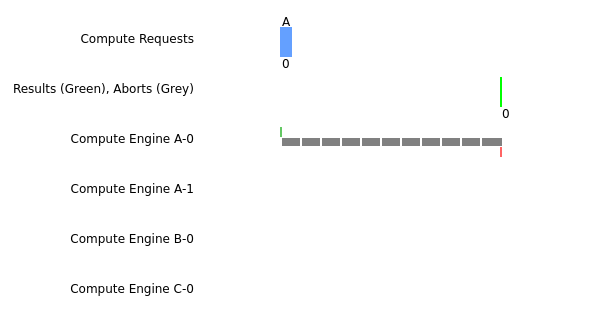
\includegraphics[width=0.8\textwidth]{figures/A}
        \caption{Suite de calculs: A}
    \end{subfigure}
    \begin{subfigure}{0.45\textwidth}
        \centering
        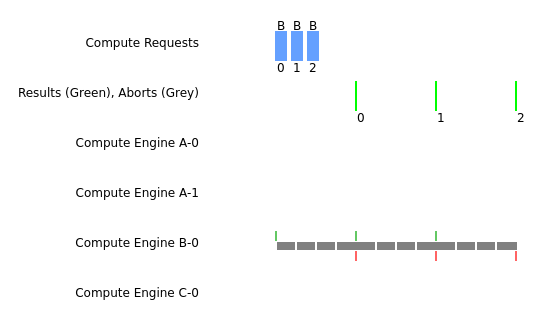
\includegraphics[width=0.8\textwidth]{figures/B_B_B}
        \caption{Suite de calculs: B, B, B}
    \end{subfigure}

    \begin{subfigure}{0.45\textwidth}
        \centering
        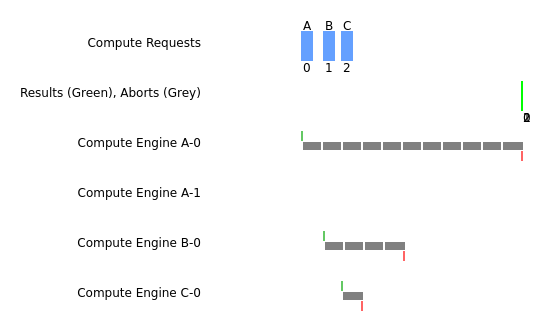
\includegraphics[width=0.8\textwidth]{figures/A_B_C}
        \caption{Suite de calculs: A, B, C}
    \end{subfigure}
    \begin{subfigure}{0.45\textwidth}
        \centering
        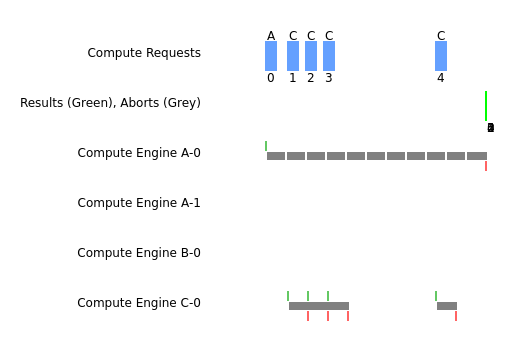
\includegraphics[width=0.8\textwidth]{figures/A_C_C_C_C}
        \caption{Suite de calculs: A, C, C, C, C}
    \end{subfigure}
    \caption{Exemple d'exécution pour l'étape 2}
    \label{fig:full2}
\end{figure}

\section{Etape 3}
Dans cette étape, nous avons mis en place la possibilité d’annuler des calculs demandés par le client grâce aux méthodes
\texttt{abortComputation} et \texttt{continueWork}.

\subsection{Choix d'implémentation}
La méthode \texttt{abortComputation} permet d’annuler un calcul en cours grâce à son identifiant. Il y a plusieurs
cas à gérer. Si le calcul n’est pas encore en cours, il faut simplement le retirer de la map \texttt{buffer}. Dans
ce cas, il faut signaler sur la condition \texttt{fullQueuePerType} que la queue pour ce type de calcul contient un
calcul en moins. Si le calcul est en cours, il faut le retirer de la liste \texttt{results} et signaler sur
la condition \texttt{notExpectedResult} pour potentiellement débloqué un thread qui attend sur ce résultat.
Si le calcul est terminé, il faut simplement le retirer de la liste \texttt{results}.
On notera qu'au vu de notre implémentation de \texttt{requestComputation}, qui ajoute directement un calcul demandé
dans la liste \texttt{results}, il faut aussi retirer le calcul de cette liste s'il est demandé mais pas encore en
cours.

La méthode \texttt{continueWork} et quant à elle assez simple, puisqu'elle va simplement chercher l'id passé en
paramètre dans la liste \texttt{results}. Si l'id est présent, cela signifie que le calcul doit continuer, sinon, cela
signifie que le calcul doit être annulé.

\subsection{Tests}
L'environnement de test comporte 3 types de calculs différents, 2 calculateurs de type \texttt{A}, un
calculateur de type \texttt{B} et un calculateur de type \texttt{C}. Les calculs de type \texttt{A} sont plus longs
que les calculs de type \texttt{B} qui sont eux même plus longs que les calculs de type \texttt{C}.
\begin{itemize}
    \item Les Google tests concernant l'étape 3 passent tous.
    \item Si on envoie une demande de calcul de type \texttt{A} et qu'on l'annule avant la fin, le calculateur s'arr
    ête et le résultat n'est pas renvoyé. C'est le comportement attendu. (Voir figure 2.a.)
    \item Si on envoie une demande de calcul de type \texttt{A} et qu'on l'annule après la fin alors que le résultat
    est déjà renvoyé, cela n'a pas de conséquence et on peut relancer un nouveau calcul. C'est le comportement attendu.
    \item Si on envoie des demandes de calcul de type \texttt{A} et \texttt{B} et qu'on annule le calcul de type \texttt{B}
    alors qu'il est déjà calculé mais avant la fin du calcul de type \texttt{A}, seul le calculateur de type \texttt{A}
    renvoie son résultat. C'est le comportement attendu. (Voir figure 2.b.)
    \item Si on envoie des demandes de calcul de type \texttt{A}, \texttt{B} et \texttt{C} et qu'on annule les
    calculs de type \texttt{B} et \texttt{C} alors qu'ils sont déjà calculés mais avant la fin du calcul de type \texttt{A},
    seul le calculateur de type \texttt{A} renvoie son résultat. C'est le comportement attendu. (Voir figure 2.c.)
    \item Lorsqu'on a annulé un calcul, on peut relancer un nouveau calcul sans problème. C'est le comportement
    attendu. (Voir figure 2.d.)
\end{itemize}

\begin{figure}[h]
    \begin{subfigure}{0.45\textwidth}
        \centering
        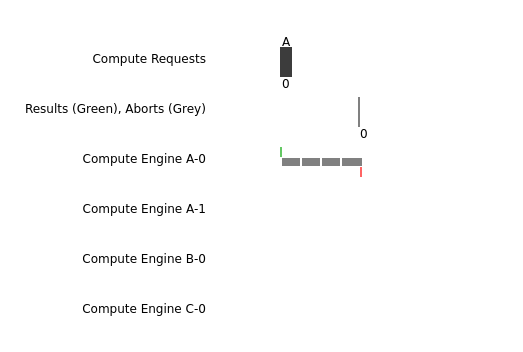
\includegraphics[width=0.8\textwidth]{figures/A_Abort}
        \caption{Suite de calculs: A abort}
    \end{subfigure}
    \begin{subfigure}{0.45\textwidth}
        \centering
        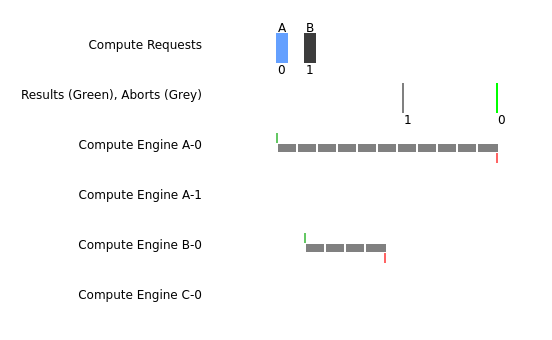
\includegraphics[width=0.8\textwidth]{figures/A_B_Abort}
        \caption{Suite de calculs: A, B abort}
    \end{subfigure}

    \begin{subfigure}{0.45\textwidth}
        \centering
        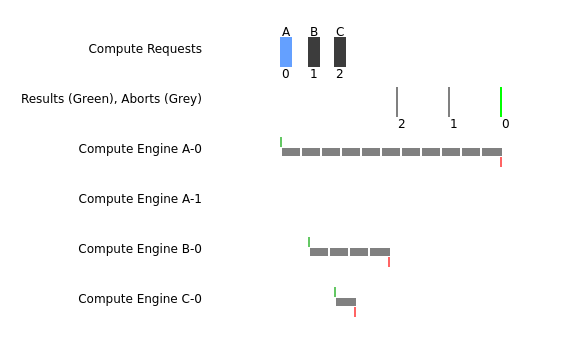
\includegraphics[width=0.8\textwidth]{figures/A_B_Abort_C_Abort}
        \caption{Suite de calculs: A, B abort, C abort}
    \end{subfigure}
    \begin{subfigure}{0.45\textwidth}
        \centering
        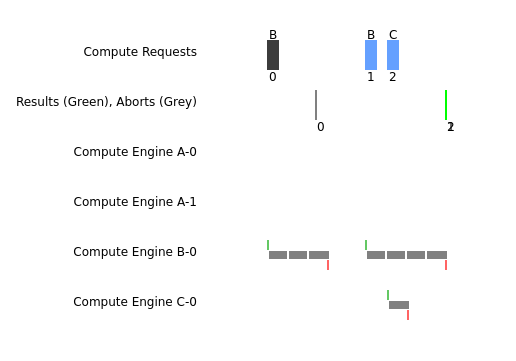
\includegraphics[width=0.8\textwidth]{figures/B_Abort_B_C}
        \caption{Suite de calculs: B abort, B, C}
    \end{subfigure}
    \caption{Exemple d'exécution pour l'étape 3}
    \label{fig:full3}
\end{figure}

\pagebreak

\section{Etape 4}
Dans cette étape, nous avons mis en place la gestion de la terminaison du buffer grâce aux méthodes \texttt{stop}
et \texttt{throwStopException}.

\subsection{Choix d'implémentation}
La méthode \texttt{stop} permet de demander l'arrêt du buffer.  Afin de modéliser
le fait que le buffer est arrêté, nous avons créé un attribut booléen \texttt{stopped} qui est innitialisé à \texttt{false}
au lancement du programme. Lorsque la méthode \texttt{stop} est appelée, on met cet attribut à \texttt{true}. De plus,
on signale sur toutes les conditions existantes dans le buffer afin de débloquer tous les threads qui attendent sur
ces dernières, afin qu'ils puissent s'arrêter.

Pour que l'arrête des threads se fasse comme attendu, nous avons dû apporter quelques modifications aux méthodes
préalablement définies. Ainsi, dans toutes les fonctions qui contiennent une attente sur une condition, nous avons
ajouté une vérification de l'attribut \texttt{stopped} avant et après l'attente sur la condition. Si on se trouve
avant l'attente et que l'attribut \texttt{stopped} est à \texttt{true}, on sort du moniteur et on lance
une exception. Si on se trouve après l'attente et que l'attribut \texttt{stopped} est à \texttt{true}, on signale sur
la condition pour débloquer les threads qui attendent dessus, on sort du moniteur et on lance une exception. Cela
permet en quelque sorte de réveiller les threads en cascade pour être sûr qu'ils s'arrêtent tous.

La méthode \texttt{continueWork} a aussi été modifiée afin de retourner \texttt{false} si l'attribut \texttt{stopped} est
à \texttt{true}, afin de signifier que le travail en cours doit s'arrêter.

\subsection{Tests}
L'environnement de test comporte 3 types de calculs différents, 2 calculateurs de type \texttt{A}, un
calculateur de type \texttt{B} et un calculateur de type \texttt{C}. Les calculs de type \texttt{A} sont plus longs
que les calculs de type \texttt{B} qui sont eux même plus longs que les calculs de type \texttt{C}.
\begin{itemize}
    \item Les Google tests concernant l'étape 4 passent tous.
    \item Les méthodes \texttt{requestComputation}, \texttt{getWork} et \texttt{getNextResult} lancent un exception si
    le buffer est arrêté si elles allaient entrer ou sortent d'une phase d'attente. C'est le comportement attendu.
    \item Lorsqu'on arrête le buffer, les threads qui attendent sur une condition sont débloqués et s'arrêtent. C'est
    le comportement attendu.
    \item Lorsqu'on arrête le buffer, tous les threads s'arrêtent (i.e on arrive à \texttt{join} sur tous les threads).
    C'est le comportement attendu.
    \item Lorsqu'on arrête le buffer, on ne peut plus ajouter/ récupérer de calculs. C'est le comportement attendu.
    \item Lorqu'on arrête le buffer, les derniers calculs sont récupérés dans l'ordre de leur demande et ne sont pas
    mélangés. C'est le comportement attendu.
\end{itemize}

\end{document}